\section{Bit Error Patterns}

We designed two experiments to investigate the results of Schmidt~\etal~\cite{Schmidt2013}, in particular the effect of temperature and hardware revision on bit error distribution.

\subsection{Effects of board layout}
\label{subsec:effects_of_board_layout}

While both versions we used are drop-in replacements for the Telos design devised by Polastre~\etal~\cite{Polastre2005}, the newer MTM-CM5000 version uses a slightly different schematic and different board layout.
Notable differences include the 3V voltage regulator and the layout of the radio circuitry.

In the experiment a pair of CM5000 and original motes transmitted to two CM5000 and two original motes.
This redundant placement shown in Figure~\ref{fig:8_mote_setup} was chosen so that the same transmission was received by both types.
Over the course of six days the four transmitters sent 563.500 messages each, totalling 2.254.000 transmitted messages at power setting 2. Of those transmitted messages a total of 5.280.369 messages were received, 2.497.744 of which had at least one bit error.
The experiment was located in a large climate-controlled server room in the basement, therefore the temperature remained within $20-25\,^{\circ}\mathrm{C}$ with no other changes in the environment.

\begin{figure}[H]
	\centering
	\begin{tikzpicture}
		\newcommand\receiver[5]{%
		    \begin{scope}[xshift=#1cm,yshift=#2cm,rotate=#3]
		        \draw[fill=#4] (0,0) rectangle (1,2.1);
		     	\draw[fill=black!10] (0.33,0.1) rectangle (0.66,-0.45);
		     	\draw[snake=snake, white, segment amplitude=1.75, segment length=5, line width=1.25pt] (0.1, 1.95) -- (0.9, 1.95);
		     	\node at (0.5cm, 1.05cm) {#5};
		    \end{scope}
		}
		\newcommand\transmitter[5]{%
			\receiver{#1}{#2}{#3}{#4}{#5};
		    \begin{scope}[xshift=#1cm,yshift=#2cm,rotate=#3]
		     	\draw[snake=expanding waves, segment angle=40, segment length=7] (0.5,2) -- (0.5,3);
		    \end{scope}
		}

		% new = red, old = blue
		% new transmitter
		\transmitter{3}{7}{-65}{motered}{0};
		\transmitter{3.675}{5.5}{-65}{motered}{1};		

		% new transmitter
		\transmitter{0}{2}{-65}{moteblue}{2};
		\transmitter{0.675}{0.5}{-65}{moteblue}{3};

		\receiver{13}{0}{180}{motered}{7};
		\receiver{13}{3}{180}{moteblue}{6};
		\receiver{13}{6}{180}{motered}{5};
		\receiver{13}{9}{180}{moteblue}{4};

		% labels
		\node at (3, 7.75) {CM5000};
		\node at (0, 2.8) {Original};

		\node at (3, -1.5) {Transmitters};
		\node at (10.5, -1.5) {Receivers};
	\end{tikzpicture}
	\caption{Experiment setup from above with four transmitters and receivers.}
	\label{fig:8_mote_setup}
\end{figure}

Note that the CM5000 motes required to be physically closer to the receivers at the same power setting to have similar link quality as the original motes.
This might be hinting at a difference in range between the two hardware layouts, however, our experiment was not setup to systematically investigate range.

In the initial evaluation we noted some significant differences in the quality of some links, were the co-located transmitters are sending to the same receiver.
For example, the link 3-5 is of very good quality with over 99\% PRR, however link 2-5 shows quite the opposite with less than 1\% PRR, even though both transmitters a located at the same distance and angle from the receiver.
This confirms the findings of Baccour~\etal~\cite{Baccour2012}, specifically that link quality is anisotropic, \ie the communication range exhibits a nonspherical pattern.
More exhibitions of this behavior can be found in the complete table of link qualifiers in the Appendix as Table~\ref{tab:8mote_link_qualities}.

Further analysis revealed the same bit and symbol error patterns as first discovered by Schmidt~\etal~\cite{Schmidt2013}, which state that within any transmitted symbol, the first three MSB are more likely to break than the LSB and that symbols with the MSB set to 1 (\ie 0x8 to 0xF) are more likely to brea.
The probability of bit errors are plotted in Figure~\ref{fig:8mote_bit_errors}, with the first 12 bytes (96 bits) consisting of the message header with partially fixed content and the remaining 80 bytes are the constant payload, made up of two 32 byte patterns of 0x0000, 0x1111, ..., 0xFFFF, and one 16 byte pattern of 0x00, 0x11, ..., 0xFF.

\begin{figure}[H]
	\subfigure[XL symbol influence.] {
    	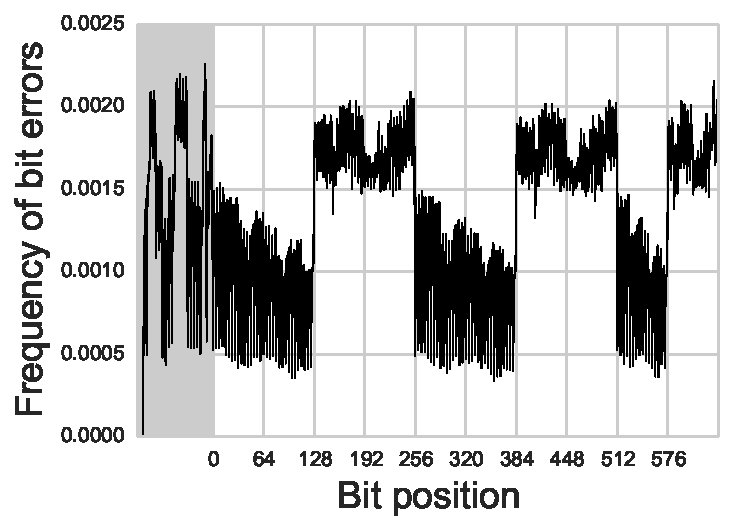
\includegraphics[width=0.5\columnwidth]{figures/8mote_0-5_xor}
    	\label{fig:8mote_bit_errors_xl}
    }
    \subfigure[L symbol influence] {
	    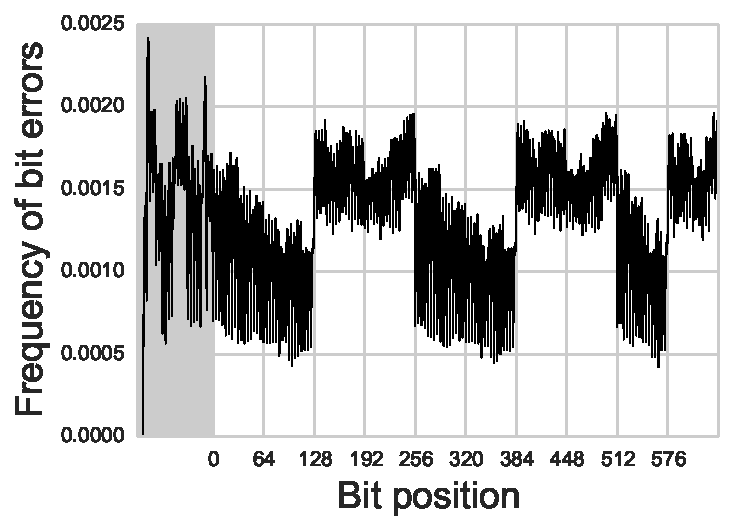
\includegraphics[width=0.5\columnwidth]{figures/8mote_1-6_xor}
	    \label{fig:8mote_bit_errors_l}
	}
	\subfigure[M influence.] {
	    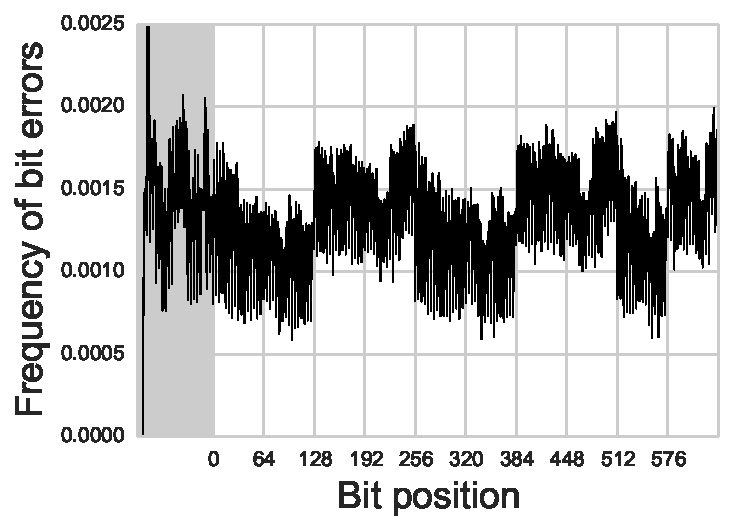
\includegraphics[width=0.5\columnwidth]{figures/8mote_2-6_xor}
	    \label{fig:8mote_bit_errors_m}
	}
	\subfigure[S influence.] {
	    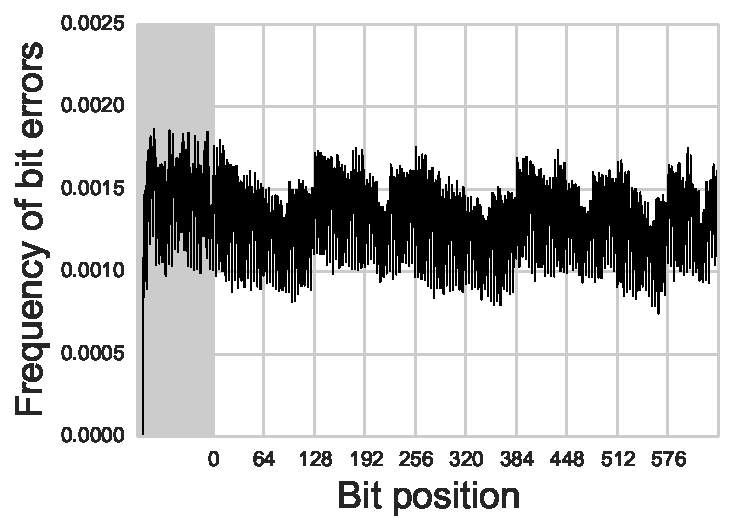
\includegraphics[width=0.5\columnwidth]{figures/8mote_2-7_xor}
	    \label{fig:8mote_bit_errors_s}
	}
	\caption{Four magnitudes of symbol content influence on bit error pattern.}
	\label{fig:8mote_bit_errors}
\end{figure}

We were able to confirm the findings of Schmidt~\etal{} and extend them with a classification of the influence of symbols on bit error probability.
The subfigures show four magnitudes of this phenomenon, ranging from and extreme to almost no difference between symbols, named XL, L, M and S.
The remaining links can be classified into these four categories as done in Table~\ref{tab:8mote_bit_error_link_classification}.

\begin{table}[H]
	\begin{tabularx}{\linewidth}{|c*{4}{|c}|}
	\hline
	\T \cellcolor{slightgray} Receiver	& \multicolumn{1}{X|}{\cellcolor{motered} \centering Sender 0} & \multicolumn{1}{X|}{\cellcolor{motered} \centering Sender 1} & \multicolumn{1}{X|}{\cellcolor{moteblue} \centering Sender 2}	& \multicolumn{1}{X|}{\cellcolor{moteblue} \centering Sender 3}\\
	\hline

	\cellcolor{moteblue}\T 4 & S  & n/a & n/a & n/a \B\\
	\hline
	\cellcolor{motered}\T  5 & XL & XL  & L   & XL  \B\\
	\hline
	\cellcolor{moteblue}\T 6 & XL & L   & M   & n/a \B\\
	\hline
	\cellcolor{motered}\T  7 & L  & n/a & S   & L   \B\\
	\hline 
	\end{tabularx}

	\caption{Classification of all links with enough bit errors (otherwise marked with n/a).}
	\label{tab:8mote_bit_error_link_classification}
\end{table}
